%\documentclass[4pt,a4paper]{article}
\documentclass[4pt,a4paper,twocolumn]{article}
\usepackage[utf8]{inputenc}
\usepackage[english]{babel}
\usepackage{algorithm}
\usepackage{textcomp}
\usepackage{fontenc}
\usepackage{tipa}
\usepackage{framed}
\usepackage{multicol}
\usepackage{color}
\usepackage{qtree}
\usepackage{graphicx}
\usepackage{amsmath}

\usepackage{cite}
\usepackage{lastpage}
\usepackage{lmodern}




\usepackage[]{hyperref}
\hypersetup{  
	colorlinks=true,
    urlcolor=cyan           % color of external links
}

\author{David Przybilla\\dav.alejandro@gmail.com, davida@coli.uni-saarland.de\\ \\ Term Paper for Unsupervised semisupervised
Learning Seminar\\ Universit\"{a}t des Saarlandes}
\title{Classification of short product reviews using semisupervised learning}
\begin{document}
\twocolumn[
	 \begin{@twocolumnfalse}
    \maketitle
  \end{@twocolumnfalse}
 ]

   \begin{abstract}
      Microblogging has become a trend,thus many users are using such platforms to share their opinions.Mining these opinions can reveal valuable information to companies, such as what features to develop in their products or marketing strategies.However there are  major drawbacks when mining tweets, first their length do not provide enough word occurrences so traditional bag-of-words methods have limitations, second they are extremely noisy and third annotated data is limited and costly to get.\\
      In this paper we address the problem of classifying short product reviews by using semisupervised learning. A comparison among two semisupervised methods and a supervised method is given. Finally we propose different ways to improve the given results by injecting knowledge into the semisupervised models.
    \end{abstract}


\section{Introduction}
Twitter and Tuenti are popular microblogging services in Latinamerica,
as prices of smartphones became more accessible to people big communities
have grown around this services.\\
These communities are actively commenting everything from political events to products experiences.\\
Therefore it has become of interest for many companies to analyze the microblogging data in order to understand
what their clients want of their products, this led naturally to sentiment Analysis.\\
\\
One of the subtasks of Sentiment Analysis is to find the topic or aspect of an opinion,
for example given a set of opinions about a mobile phone, it is possible to label each comment
with the topic that it is referring to, this labels could be ``battery", ``design", ``operative system" etc.
This Subtask can be modelled as a classification problem, given a set of fixed possible topics.\\
\\
In the scenario of text classification semisupervised techniques present two advantages:\\
First a semisupervised method should allow to classify text by annotating only a small portion of data,thus reducing the labor of annotating.\\
Second the unlabelled data is used during training, this is important since the amount of unlabelled data in these tasks is abundant and available, therefore it can be used to provide extra knowledge to the model.\\
\\
Zhang and Kubota ~\cite{Ando:2005:FLP:1046920.1194905} proposed a semisupervised approach using linear classifiers for multiple learning tasks.\\
They proposed to create additional classifications tasks (Auxiliary Problems) aside from the Target Problem.\\
The underlying idea is that the auxiliary problems will help finding good predictive structures.\\
One of the constraints in this approach is that auxiliary problems should be  able to automatically generate labelled data from the original unlabelled data.
This method has been used in tasks such as Text Chunking ~\cite{Ando:2005:HSL:1219840.1219841}\\
\\
In contrast ~\cite{Zhu:2005:SLG:1104523} proposes a graph approach called label propagation for
doing semisupervised learning.\\
This approach maps the data to a graph representation, then labelled instances propagate their labels through the graph, allowing unlabelled data to adopt the label of those instances which are similar.\\
~\cite{Speriosu_twitterpolarity} uses Label Propagation for doing Polarity Classification on tweets.\\
\\
Even though classifying text has been a widely studied topic,the focus has been on long documents,
whereas tweets are at most 144 characters long.\\
The new trends in these social networks have led to research about classification in short texts, the latter has  shown that it arises new challenges, and former approaches are not  effective.\\
One of the reasons is that  user generated comments in the mentioned services tend to be extremely short, leading to sparce feature representations.\\
\\
In respect to short text classification Xinghua and Hongge ~\cite{Fan:2010:NMC:1916732.1917677} proposes  to do Feature Extension to deal with data sparcity, in their approach each comment is extended with extra words from an expansion vocabulary.\\
~\cite{Gabrilovich:2006:OBB:1597348.1597395} proposes on the other hand to use encyclopedic knowledge from wikipedia for extending the short comments.\\
As opposed to the above ones,  ~\cite{Sun:2012:STC:2348283.2348511} reduces the word space of the comments to keywords and use information retrieval with a voting scheme to find labels for short comments.\\
\\
This paper describes the setup of an experiment for classifying short-text comments of product reviews extracted from twitter.\\
Two semisupervised techniques are used, Label Propagation ~\cite{Zhu:2005:SLG:1104523}  and  a variation of Structural learning problem for multitasks ~\cite{Ando:2005:FLP:1046920.1194905}.\\
The next sections describe briefly  the preprocessing of the tweets,each of the proposed semisupervised methods and how they were adapted to the task. \\
Addionally the results are shown, where both methods are compared among themselves and to a supervised approach.
Finally a short conclusion and future work are discussed.\\
\\
The source code of the implementation is available at github\footnote{\url{https://github.com/dav009/LPForTopicIdentification}},the datasets however are not public, since they are constrained by a permission license.

\section{Datasets}
The Datasets of this experiments were provided by Meridean.\\
Meridean\footnote{\url{http://merideangroup.com/}} is a Colombian company which extracts tweets
mentioning latinamerican companies or products.\\
\\
The datasets are separated by product.\\
There are 3 datasets in this experiment:
\begin{itemize}
	\item Sportswear dataset
	\item Mobile-Phone dataset
	\item Hygienic-product dataset
\end{itemize}

Each dataset is composed of tuples,each tuple contains : the source of the opinion, the opinion, the polarity and the topic.\\

\begin{table}[h]
\centering
\begin{tabular}{| l |}
\hline
\textbf{Comment:}\\
$\#$ProbandoXperiaArcS Gracias @TalkMex.\\
Las fotos se ven tan nitidas.\\
\hline
\textbf{Translation:}\\
$\#$TestingXperiaArcs Thanks to @TalkMex.\\
Pictures are very sharp.\\
\hline
\textbf{Topic:}\\
Camera\\
\hline
\end{tabular}
\caption{Sample Comment}
\label{tab:sampleTuple}
\end{table}

Each dataset contains approximately 5000 tuples.

\section{Pre-processing}

The Datasets used in this experiment are actual data crawled from twitter and other sources, therefore there is a lot of noise in them.\\
Some of the problems are (but not limited) to:\\
\begin{itemize}
	\item Miss spelled words, from typo errors to lack of accents.
	\item Internet Language, replacing some letters for others whose phonetics are similar i.e: ``\textbf{qu}iero" (I want) for ``\textbf{k}iero", abbreviations and expressions (``Jaja'' ``jiji" ... )
	\item Twitter Jargon such as: ``RT:",``@"..
\end{itemize} 

The pre-processing done was the following:
\begin{enumerate}
	\item Remove Strange characters, such as hearts, and other unicode characters
	\item Remove some of the Twitter Jargon 
	\item Use \href{http://www.ims.uni-stuttgart.de/projekte/corplex/TreeTagger/}{TreeTagger} ~\cite{Schmid94probabilisticpart-of-speech} for getting the part of speech and the stem of each word in each comment
	\item discard those words that are not adjectives, nouns or verbs
	\item replace each word by its stem in lowercase
	\item remove accents from words
\end{enumerate}

When it comes to pre-processing there could be a wide number of possible 
tasks that can be done, I try to keep it simple given the time constraints. \\
\\
As a result of this pre-processing each comment is converted into a bag of keywords.\\
This will be later transformed into a vector space representation.




\section{Label Propagation}

This semisupervised learning graph method was proposed by Zhu ~\cite{Zhu:2005:SLG:1104523}.\\
The idea behind Label propagation is similar to K-Neighbours, nevertheless Label Propagation make use of the unlabelled data during the training process.\\

This approach maps the data to a graph representation.
In this representation each arc of the graph will connect two nodes only if the two nodes are similar,
the weights of the arcs are directly proportional to the similarity of the incident nodes.\\

With respect to our classification task,each node in the graph corresponds to the feature vector of a comment.
The weights of the arcs are given by the cosine distance among the vectors.\\
The final representation is a complete graph.\\
\\
In the LP algorithm, the label information of any
node in a graph is propagated to nearby nodes
through weighted arcs until a global stable stage is
achieved ~\cite{Chen:2006:REU:1220175.1220192}.
If a weight arc is high, the label will travel easier through the graph.\\
\\
The LP Algorithm iterates until convergence,
at each step the algorithm will push the labels
of the labelled data points through the arcs of high weights.The underlying assumption is that instances among a class will have high weighted arcs
connecting them.\\
At each iteration the labels of the labelled data are clamped.\\

This propagation is done by measuring a transition matrix $T$.
The transition matrix states the probability of propagating the label of an instance,
and it is measured from the weights of the arcs of the graph.\\
\\
Let $T_{ij}$ be the probability of propagating the label of instance $i$ to instance $j$, then it can be defined as:\\
\begin{align}
	T_{ij}=P(i \rightarrow j)=\frac{w_{ij}}{\sum_{k=1}^{n} w_{kj}}
\end{align}

\subsection{Algorithm}
Let $Y_{ij}$ be the soft probability of labeling instance $i$ with label $j$.\\
\\
Given our semisupervised task, then $Y$ can be divided into:\\
\\
$Y_{U}$:the soft labels for the unlabelled data\\
$Y_{L}$:the soft labels for the labelled data\\
\\
This means that $Y_{L}$ is given at the beginning of the problem
and the target is to find good values for $Y_{U}$.\\
\\
\textbf{Step 1 - Init}: In this step, the labels for $Y_{L}$ are clamped, and the labels for $Y_{U}$ are randomly initialized.\\
The proof that the initialization values of $Y_{U}$ are not transcendental can be found at ~\cite{Zhu:2005:SLG:1104523}.\\
\\
\textbf{Step 2 - Propagation}: In this step, the labels of neighbouring nodes are pushed.\\
Let $t$ be the current iteration, then $Y^{t+1}$ is defined as:
\begin{align}
Y^{t+1} = T Y^{t}
\end{align}
\\
\textbf{Step 3 - Clamp Labelled Data}: In this step, the Labels for $Y_{L}$ are clamped.\\
\\
\textbf{Step 4 - Repeat}: Repeat from step 2 until convergence.\\
\\
\textbf{Step 5 - Labeling Approach}: Once there is convergence, a label has to be chosen for each node in the graph, there is more than one approach.\\
The simplest approach would be to pick the label with the highest probability. \\
In ~\cite{Zhu:2005:SLG:1104523} there is an empirical analysis on more sophisticated approaches, there it is shown how this criteria can affect the performance, nevertheless for this experiment the simple approach was used.\\
\\
More sophisticated versions of this approach have been presented and assessed, in ~\cite{Talukdar:2010:EGS:1858681.1858830} Talukdar and Pereira showed an empirical comparison among different variations of the LP algorithm, a modified absorption algorithm is presented where seed labels are not clamped,and it is shown to have better performance in the given tasks.
Nevertheless within this paper we call LP to the algorithm proposed by Zhu ~\cite{Zhu:2005:SLG:1104523}.\\
\\
To summarize in our experiment we convert our data into a complete graph,
each node is the feature vector of a comment, and the weight of each arc
corresponds to the similarity of the comments being incident to the arc.\\
This Graph is  fed to the Label Propagation Algorithm proposed by Zhu.\\



 
\section{Structure Learning}
A semisupervised learning method proposed in ~\cite{Ando:2005:FLP:1046920.1194905}.\\
This paper proposes a way to learn multiple classification tasks.In this approach the original Classification Task(Target Problem) is extended by creating a set of auxiliary classification tasks.\\
The auxiliary classification tasks are used to improve performance on the target task,
the underlying assumption is that by solving the auxiliary problems one should be able to find good predictive structures.\\
The Auxiliary Tasks are trained on the unlabelled data,in consequence one constraint to the creation of auxiliary tasks is that they should be able to automatically generate training data from the target's problem unlabelled data.In ~\cite{Ando:2005:HSL:1219840.1219841} it is argued that having a high number of auxiliary tasks is beneficial for the performance.\\
\\
In this paper's experiment, the target task corresponds to find the topic of each comment.\\
The auxiliary problems are defined as:\\
learning a linear predictor using the Unlabelled data for the $K$ most common words in the unlabelled data and a predictor for the words with highest Pointwise mutual information(PMI) from the labelled Data.\\
By doing this, both the features of the labelled data and unlabelled data will be extended, the labelled data will be extended with features from the unlabelled data, and the unlabelled data will be extended with predictive features of the labelled data.\\
\\
For learning this tasks, first the words with highest PMI are found using the labelled data, then the words with highest frequency in the unlabelled data are found.\\
Subsequently a linear classifier for predicting each of the most common words is trained using the unlabelled data, and a linear classifier for predicting each of the most predictive words is trained using the labelled data.
It is clear that labels for this tasks can be easily generated by masking the words for which the classifiers are being trained to predict.\\
\\
By solving the auxiliary tasks, the feature vectors of the training data for the target problem can be extended with the predictions of the auxiliary tasks.Also the vectors of the unlabelled data are extended.\\
This might shown useful in the setup of the experiment, since we are extending the feature representations from knowledge of unlabelled data.\\
\\
Finally a linear classifier is learnt using the training data for the target problem.\\
With respect to the ASO-SVD algorithm, this paper just explore a naive approach by using auxiliary problems, in this regard the auxiliary classifiers are used to extend the feature vectors.\\
For the rest of the paper we will refer to this approach as Naive SL.


\section{Experiment}
For the experiments, the three datasets mentioned above were used as training and test data.\\
The experiments corresponds to the following:
\begin{itemize}
	\item Single task Supervised Learning using SVM ($SVM$)
	\item Single task semisupervised Learning using Label Propagation ($LP$)
	\item Single task semisupervised Learning using The naive Structural Learning($SL$)
	
\end{itemize}

Each of the experiments were ran with different amounts of training data, specifically 10\%, 30\%, 60\% and 90\%\\
\\
For the Label Propagation  $Junto$ \footnote{ \url{https://github.com/parthatalukdar/junto} } ~\cite{Talukdar:2010:EGS:1858681.1858830} was used. $Junto$ is an open source implementation of the Label Propagation algorithm.\\
\\
For $SL$ and $SVM$ the libsvm\footnote{\url{http://www.csie.ntu.edu.tw/~cjlin/libsvm/}} library provided an implementation for training SVM.\\
For all the linear classifiers trained in the experiments a  Polynomial Kernel was picked and the value of $gamma$ was 1.2, the reason behind this choice is motivated by the empirical results obtained by ~\cite{Joachims:1998:TCS:645326.649721} in a similar task.\\
\\
For making the tasks suitable for the given computational power, a subset of the size of $\frac{1}{4}$ of each of the given datasets was used, this has a major drawback, since the more the data the better the behaviour of the semisupervised algorithms.
Furthermore an upper bound on the number of auxiliary classifiers created by  the naive structure learning was imposed, the auxiliary problems would be 40\% of the most common words in the unlabelled data and the words with highest PMI from the Labelled data.\\
A major drawback of Label Propagation from a running time perspective is having to calculate a complete graph containing the similarity among the nodes.Calculating a graph with 2 or more millions of arcs consume lots of resources.
\section{Results}
In overall the Naive SL could maintain the f-score given by the supervised approach, in some cases was able to get a much better f-score by improving recall, in some other cases a slightly better recall resulted in a decline of the precision thus leading to a worse f-score.\\
\\
The LP approach on the other hand raised in labels where both of the previous approaches failed such as with the label $Resistance$  in the sportswear dataset Figure~\ref{fig:nike_90_fscore} or $Brand$ $Support$ Figure~\ref{fig:nike_10_fscore},  $Tenderness$  in the Hygienic Product dataset Figure~\ref{fig:terra_30_fscore}, and many others like $Photography$,$Screen$ and $Social$ $Networks$ in the Mobilephone dataset Figure~\ref{fig:sony_30_fscore_more}.\\
\\
The Hygienic Product and Sportswear datasets shown some decent results, whereas the Mobile Phone dataset shown to be challenging.\\
\\
One factor that might have affected the overall performance was using a subset of the data, this specially seems to affect LP.\\
LP profits from abundant unannotated data, my hypothesis is that using a very small set of seeds with a large number of unannotated data should improve the scores given below.\\
The reason for LP giving such low scores  on some of the tasks might be caused by the limitation on the dataset sizes and the data sparsity in the feature vectors.\\
\\
First the Limitation on the size of the datasets might have caused a lack of extra samples, thus  generating some disconnected segments of the graph in case of LP, therefore a proper propagation could not be carried out successfully for prediction.\\
\\
Second the feature vectors are very sparse, because of the bag of keywords approach and the short text nature of the task, thus leading also to disconnected segments of the graph.\\
\\
A second test was carried out in an attempt to discover whether both more data and selecting more features would benefit the approach, this second test was done on the Mobile Phone dataset.\\
In this trial more data were taken into account and a larger number of features were allowed to be part of the feature vectors,this would also benefit SL since the number of auxiliary problems would be incremented.
The results are given in Figure~\ref{fig:sony_10_fscore_more} and Figure~\ref{fig:sony_30_fscore_more}, in general it can be said that there is much a better f-score for a larger number of labels when compared to the previous tests, so It is possible to speculate that using the whole datasets would greatly increase the f-scores given in this report.\\
\\

Since comments are reduced to a bag of keywords other factors which could have caused the given results are:
\begin{itemize}
\item \textbf{Noise}:the given data is actual user-generated content thus very noisy.\\
Noisy data such as miss written words can lead to bad classifications or points isolated in the LP graph. Take as an example the label $Camera$ for the Mobile phone dataset, if a good predictor for this label is the actual word ``camera" and this word has been seen in the labelled data, seeing variations such as ``camraa" might not result predictive, since they would be in a different dimension.

\item \textbf{Sparsity and Short Text}: feature vectors are very sparse and text is short. This could affect in the following ways, lets think again on the label $Camera$ for the Mobile  phone dataset, if we assume we are classifying long texts, an annotated instance can reveal a lot of the topic vocabulary , in this case words such as ``resolution", ``megapixels" and so on.\\
On the other hand in the short text classification, you got at most 144 characters per text, so you might end up only with a small subset of topic related words.
For example lets assume you have a set of good predictors in your labelled data and those predictors are the words: ``Camera" and ``resolution".If there is a comment saying just: ``it has a good amount of megapixels", it will be very unlikely to be classified correctly, unless there is another comment linking ``megapixels" with one of the predicting words in the seed set.\\
\\
With respect to the topic vocabulary, I would speculate that this really affect the performance. In the Hygienic Product and  Sportswear the term's range are more or less reduced, this is not the case of the mobile phone dataset, the range of topic vocabulary for each label is huge, just take into account the label $Application$, a comment can be given this label if it has a mention to a well known IOS or Android App, such as ``Angry Birds", furthermore take into account the label $Social$ $Network$ where social networks' names are mentioned. On top of that combine all the possible technical words that might appear with the labels $Camera$, $OS$, $Photography$.

\end{itemize} 



\section{Conclusions and Future Work}
An experiment on classifying short comments about products was described, two semisupervised approaches were presented and compared for solving this problem.\\
\\
Data sparsity and the length of the texts shown to be an issue for Label Propagation.
One idea for tackling this problem would be to try injecting some knowledge related to the labels, this could be useful in the difficult tasks such as the Mobile Phone dataset.An approach similar to the one given by ~\cite{Gabrilovich:2006:OBB:1597348.1597395} could be tried.Basically Wikipedia could be used to gather Topic vocabulary and use that vocabulary to extend each of the comments, this could solve disconnected segments in the graph.\\
\\
Another idea worth trying is to use the SL for multitask classification instead of tackling each dataset by separate, it might be beneficial  to  join them and solve them as a single classification problem.However this requires more computational power but  at the same time it should allow better results.\\
\\
In spite of noise being a problem, I would speculate that given enough data the problem of noisy entries such as miss-spelled words should not be a big issue, this assuming there is enough noisy data in both the labelled and unlabelled entries.\\
\\
It would be also interesting to try the other Label Propagation variations such as Modified Adsorption (MAD) discussed in ~\cite{Talukdar:2010:EGS:1858681.1858830}, these implementations are available in Junto.\\
MAD should help when dealing with noisy input labels, which was one of the cases between $Photography$ and $Camera$ in the Mobile Phone dataset.\\
\\
Finally considering joining the naive SL given here with LP should help the latter to get better scores, this by allowing to connect some of the isolated sub-graphs generated by the feature sparsity.


%other LP variations ( MAD for noisy ..)
%multitask
%more feautures for running
%extending the comments with extra knowledge
%better preprocesing

\bibliography{paper}{}
\bibliographystyle{alpha}





\begin{figure*}[]
  
  \centering
    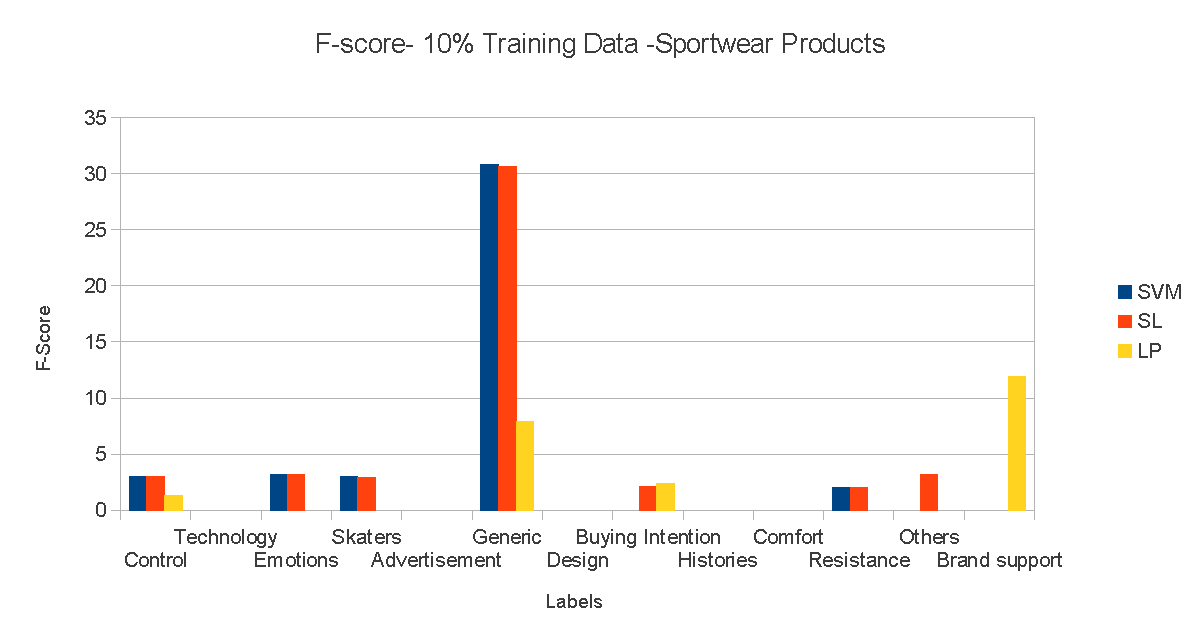
\includegraphics[scale=0.7]{graphics/sportWear/fscore-10-nike}
    \caption{F-Score, 10\% Training Data, Sportwear dataset}
   \label{fig:nike_10_fscore}  
\end{figure*}

\begin{figure*}[]
  
  \centering
    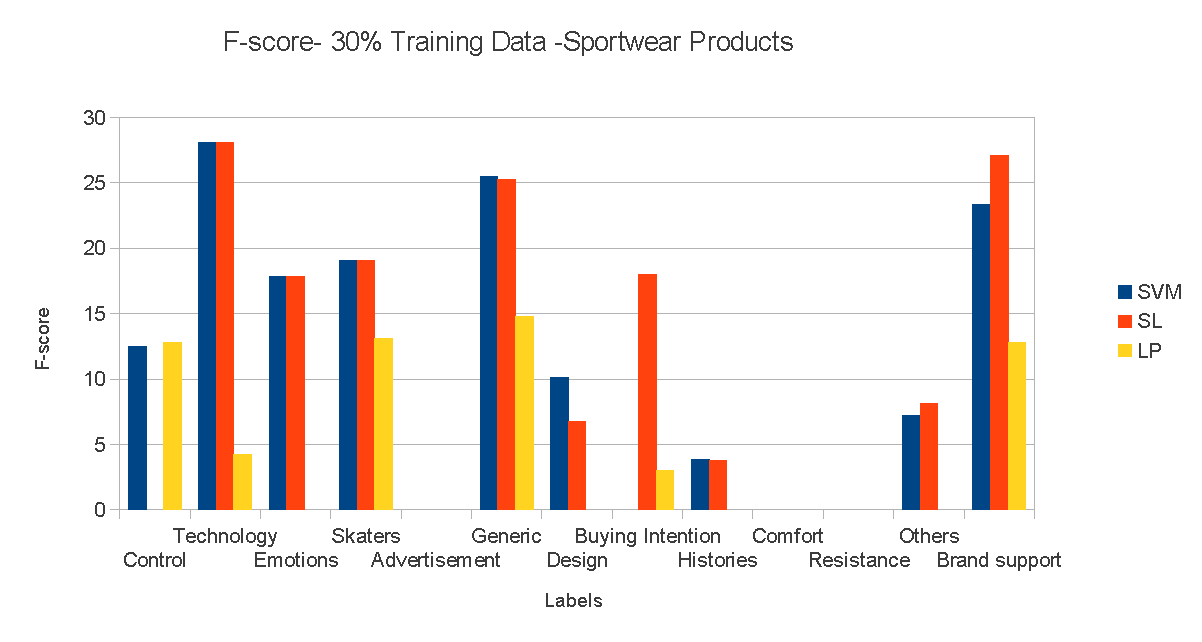
\includegraphics[scale=0.7]{graphics/sportWear/fscore-30-nike}
    \caption{F-Score, 30\% Training Data, Sportwear dataset}
   \label{fig:nike_30_fscore}  
\end{figure*}


\begin{figure*}[]
  
  \centering
    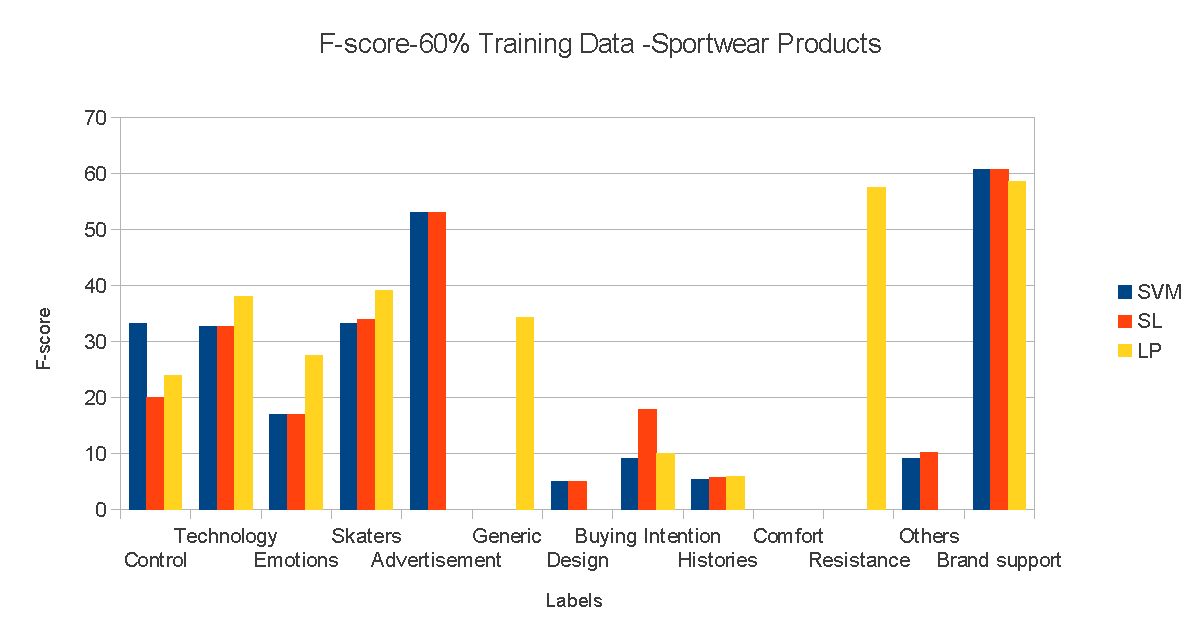
\includegraphics[scale=0.7]{graphics/sportWear/fscore-60-nike}
    \caption{F-Score, 60\% Training Data, Sportwear dataset}
   \label{fig:nike_60_fscore}  
\end{figure*}

\begin{figure*}[]
  
  \centering
    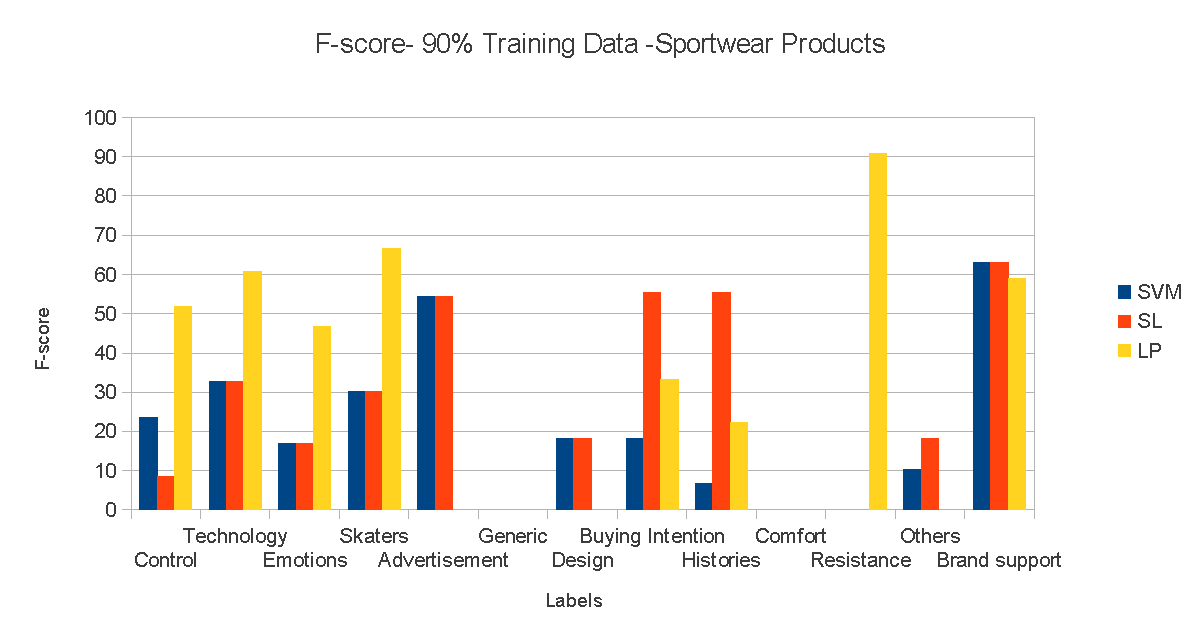
\includegraphics[scale=0.7]{graphics/sportWear/fscore-90-nike}
    \caption{F-Score, 90\% Training Data, Sportwear dataset}
   \label{fig:nike_90_fscore}  
\end{figure*}


\begin{figure*}[]
  
  \centering
    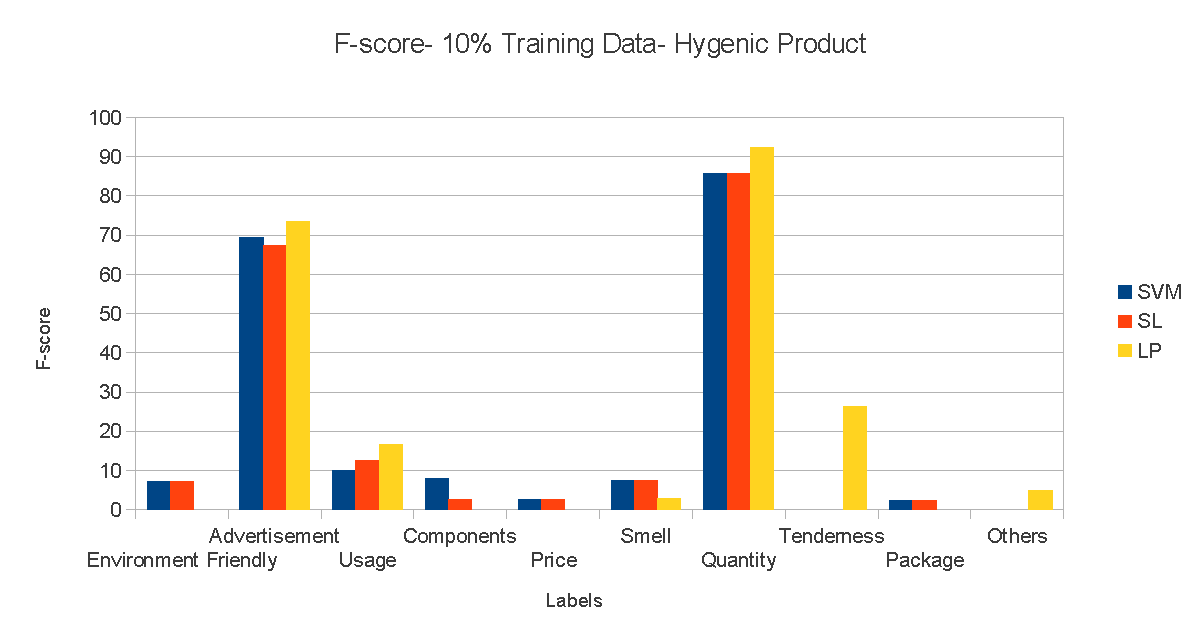
\includegraphics[scale=0.7]{graphics/terra/fscore-terra-10}
    \caption{F-Score, 10\% Training Data,Hygienic Product}
   \label{fig:terra_10_fscore}  
\end{figure*}


\begin{figure*}[]
  
  \centering
    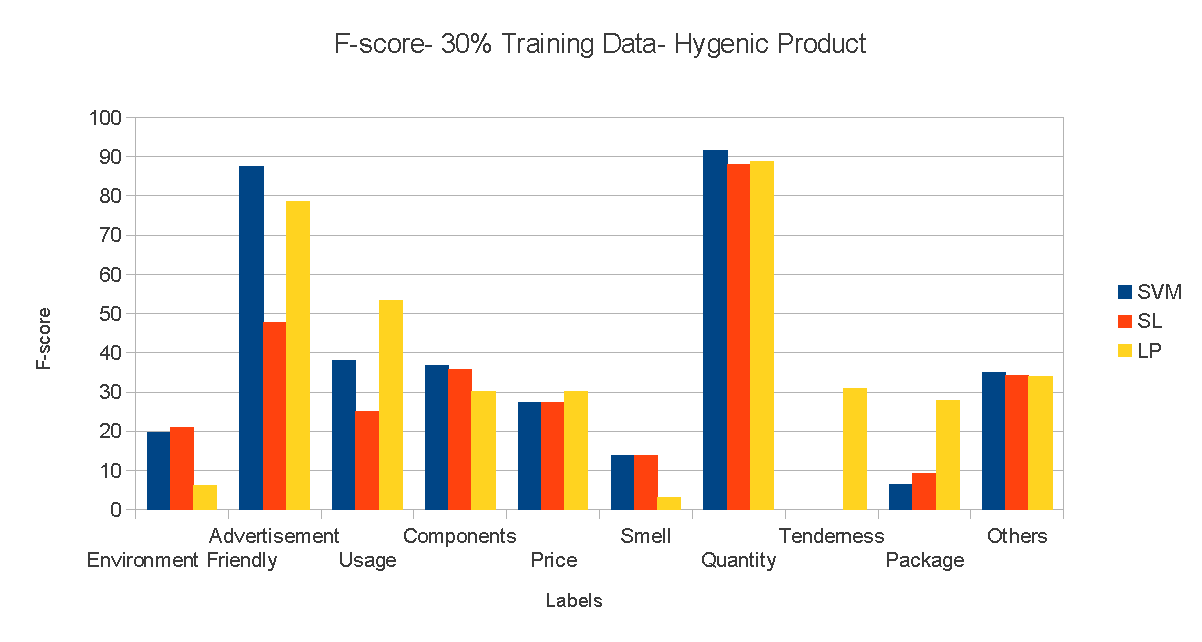
\includegraphics[scale=0.7]{graphics/terra/fscore-terra-30}
    \caption{F-Score, 30\% Training Data, Hygienic Product}
   \label{fig:terra_30_fscore}  
\end{figure*}




\begin{figure*}[]
  
  \centering
    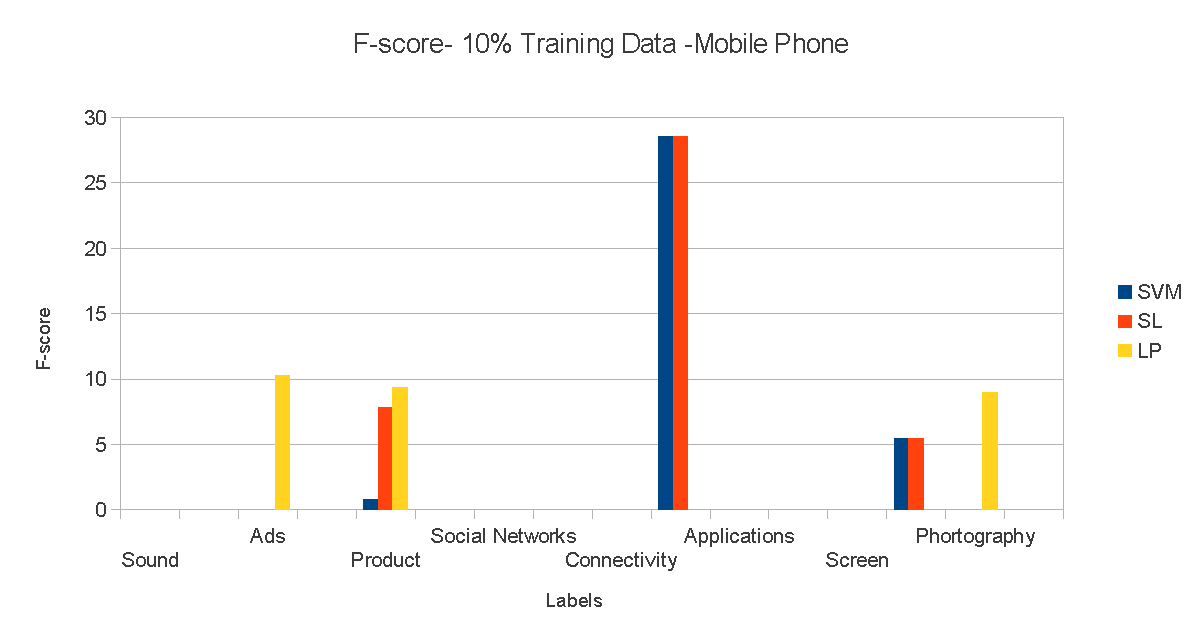
\includegraphics[scale=0.7]{graphics/sony/halfData/fscore-10-sony}
    \caption{F-Score, 10\% Training Data, Mobile Phone dataset}
   \label{fig:sony_10_fscore_half}  
\end{figure*}

\begin{figure*}[]
  
  \centering
    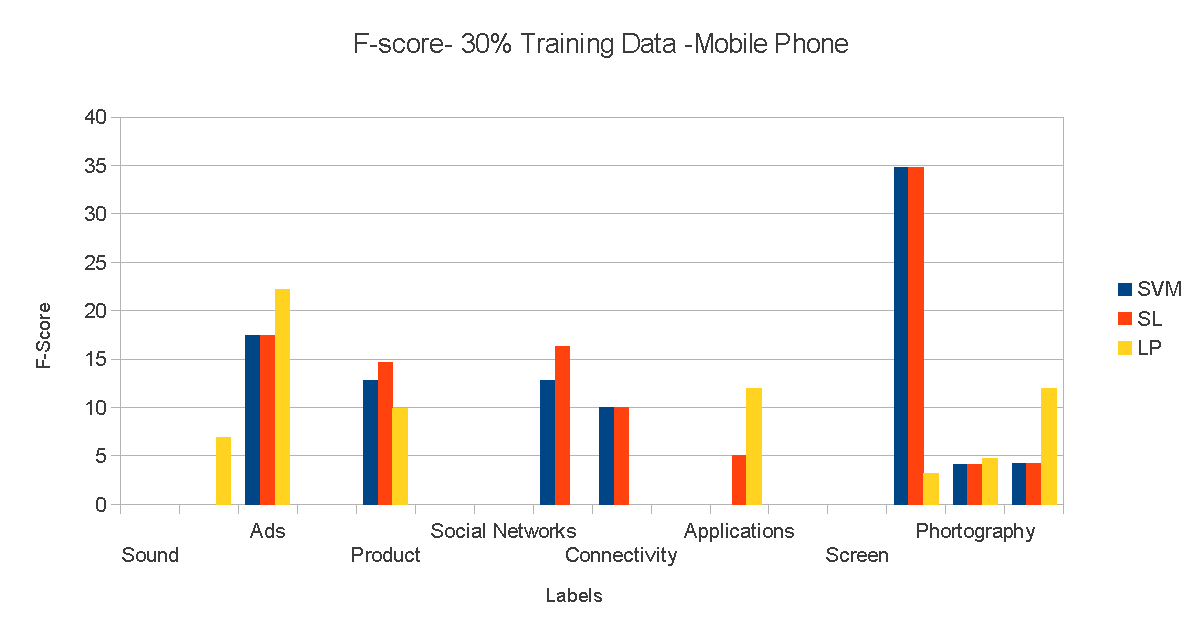
\includegraphics[scale=0.7]{graphics/sony/halfData/fscore-30-sony}
    \caption{F-Score, 30\% Training Data, Mobile Phone dataset}
   \label{fig:sony_30_fscore_half}  
\end{figure*}

\begin{figure*}[]
  
  \centering
    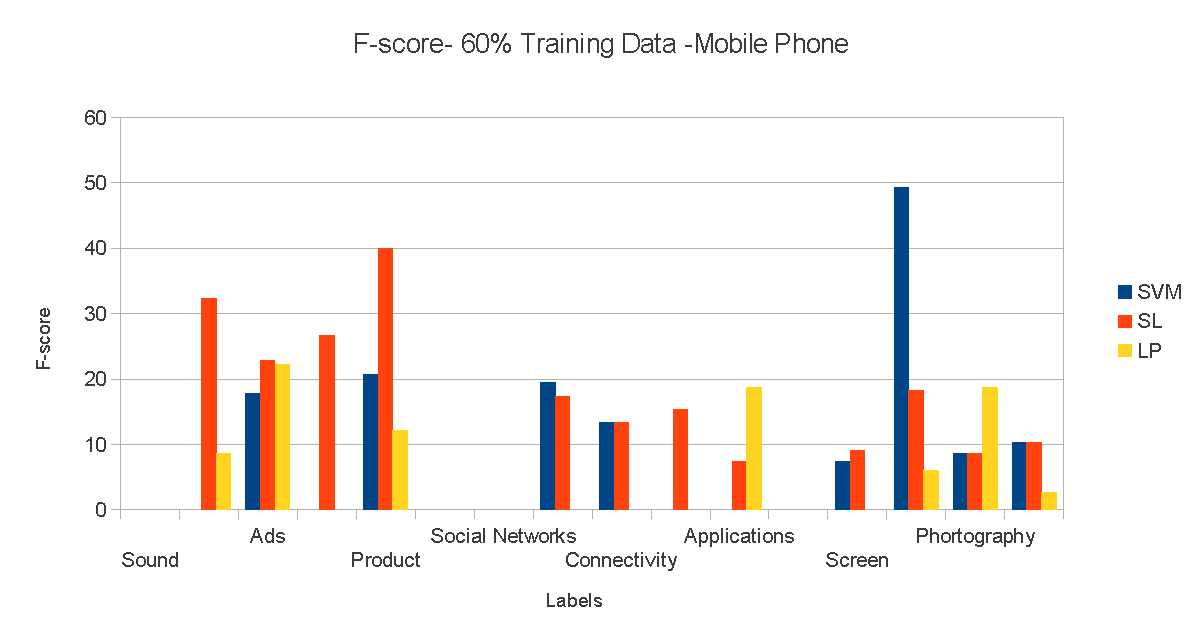
\includegraphics[scale=0.7]{graphics/sony/halfData/fscore-60-sony}
    \caption{F-Score, 60\% Training Data, Mobile Phone dataset}
   \label{fig:sony_60_fscore_half}  
\end{figure*}


\begin{figure*}[]
  
  \centering
    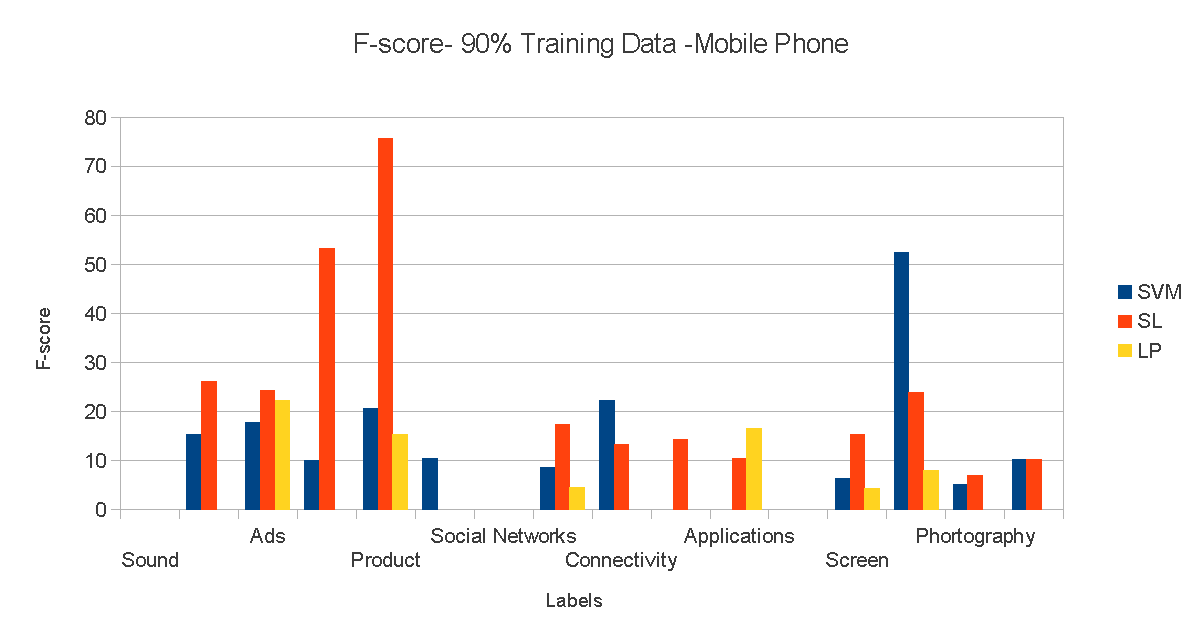
\includegraphics[scale=0.7]{graphics/sony/halfData/fscore-90-sony}
    \caption{F-Score, 90\% Training Data, Mobile Phone dataset}
   \label{fig:sony_90_fscore_half}  
\end{figure*}



%more data!

\begin{figure*}[]
  
  \centering
    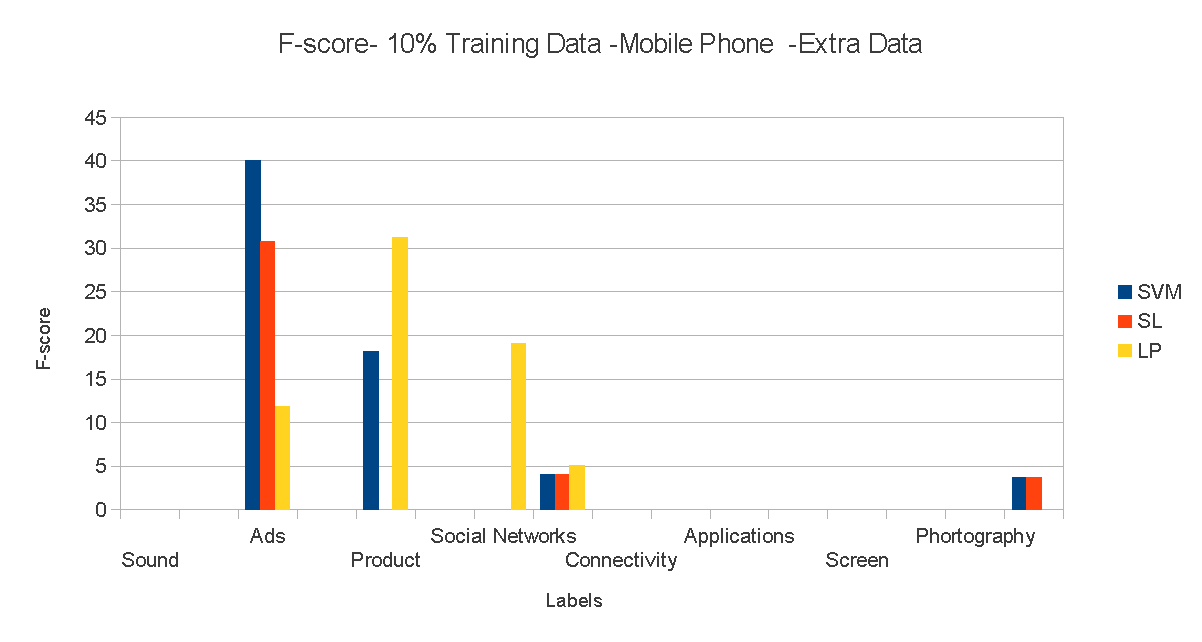
\includegraphics[scale=0.7]{graphics/sony/moreData/fscore-10-sony}
    \caption{F-Score, 10\% Training Data, Mobile Phone dataset, More Features and Data}
   \label{fig:sony_10_fscore_more}  
\end{figure*}

\begin{figure*}[]
  
  \centering
    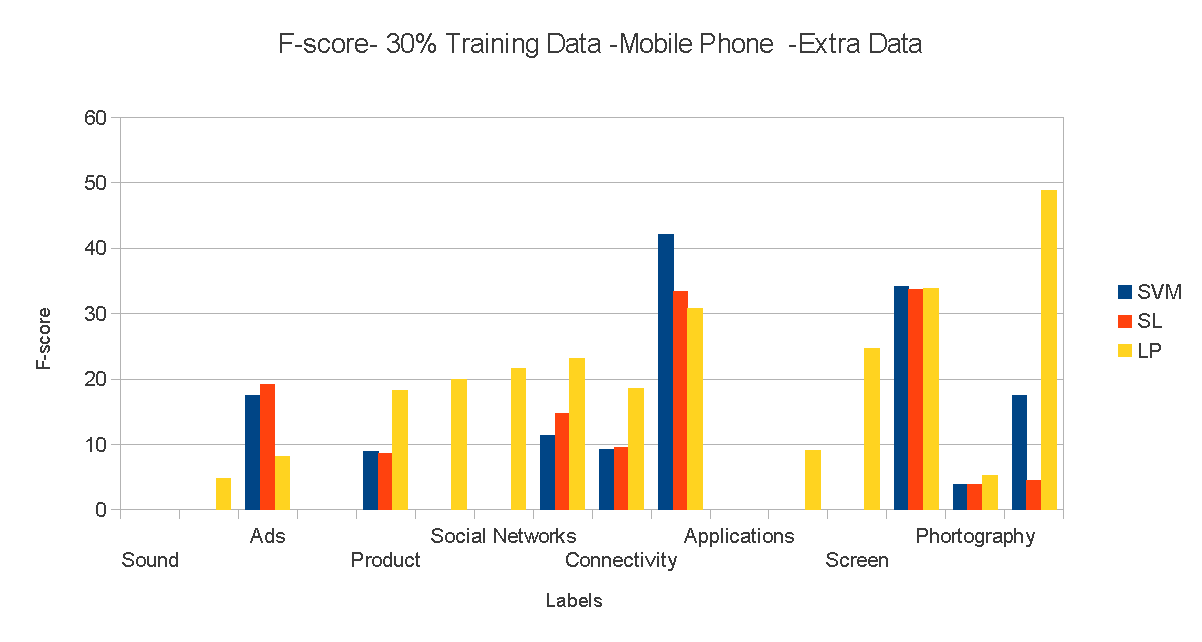
\includegraphics[scale=0.7]{graphics/sony/moreData/fscore-30-sony}
    \caption{F-Score, 30\% Training Data, Mobile Phone dataset,More Features and Data}
   \label{fig:sony_30_fscore_more}  
\end{figure*}


\end{document}


